\documentclass[12pt]{extreport}
\usepackage{subfigure}
\usepackage[utf8]{vietnam}
\usepackage[left=2.00cm, right=2.00cm, top=3.50cm, bottom=3.00cm]{geometry}
\usepackage{fancybox,graphicx}
\usepackage{mathrsfs} 
\usepackage{amsfonts}
\usepackage{longtable,array}
\usepackage{multirow}
\newlength\mylength
\newcolumntype{C}[1]{>{\centering\arraybackslash}p{#1}}
\usepackage[intlimits]{amsmath}
\usepackage{array}
\usepackage[unicode]{hyperref}
\usepackage{algorithm}
\usepackage{algorithmicx}
\makeatletter
\renewcommand{\ALG@name}{Thuật toán}
\makeatother
\usepackage{algpseudocode}
\usepackage{amsxtra,amssymb,latexsym,amscd,amsthm}
\usepackage{enumitem}
\usepackage{tikz}
\usetikzlibrary{shapes.geometric}
\usetikzlibrary{positioning,automata}
\usepackage{scrextend}
\usepackage{longfbox}
\usepackage{indentfirst}

%Môi trường Lời giải
%\newtheorem{theorem}{Định lý}[chapter]
%\newtheorem{definition}{Định nghĩa}[chapter]
%\newtheorem{example}{Ví dụ}[chapter]
%\newtheorem{lemma}[theorem]{Bổ đề}
%Tiêu đề
\newtheorem{pro}{Bài toán}
\newtheorem*{constr}{Ràng buộc}
\newtheorem*{calfunc}{Các hàm được thực thi}
\newtheorem*{Sol}{Giải thuật}
\newtheorem*{Anal}{Phân tích giải thuật}

\usepackage{fancyhdr}
\pagestyle{fancy}
\lhead{}
\chead{}
\rhead{Báo cáo Design Pattern}
\lfoot{}
\cfoot{\thepage}
\rfoot{}

\usepackage{multicol}
\setlength{\columnsep}{1cm}
\usepackage{xcolor}
\usepackage{listings}

\definecolor{mGreen}{rgb}{0,0.6,0}
\definecolor{mGray}{rgb}{0.5,0.5,0.5}
\definecolor{mPurple}{rgb}{0.58,0,0.82}
\definecolor{backgroundColour}{rgb}{0.95,0.95,0.92}

\lstdefinestyle{CStyle}{
	backgroundcolor=\color{backgroundColour},   
	commentstyle=\color{mGreen},
	keywordstyle=\color{magenta},
	numberstyle=\tiny\color{mGray},
	stringstyle=\color{mPurple},
	basicstyle=\footnotesize,
	breakatwhitespace=false,         
	breaklines=true,                 
	captionpos=b,                    
	keepspaces=true,                 
	numbers=left,                    
	numbersep=5pt,                  
	showspaces=false,                
	showstringspaces=false,
	showtabs=false,                  
	tabsize=2,
	language=C
}
\usepackage{subfigure}
\usepackage{wrapfig}
\begin{document}
%% thêm trang bìa vào
\thispagestyle{empty}
\thisfancypage{
	\setlength{\fboxsep}{5pt}
	\shadowbox}{}

\begin{center}
	
	{\fontsize{13pt}{1}\selectfont\textbf{ĐẠI HỌC QUỐC GIA HÀ NỘI}}
	\\
	{\fontsize{13pt}{1}\selectfont\textbf{TRƯỜNG ĐẠI HỌC KHOA HỌC TỰ NHIÊN}}
	\\	
	\textbf{--------------------  o0o  ---------------------}\\[1cm]
	
\includegraphics[scale=0.25]{GALLEYS/Logo-DH-Khoa-Hoc-Tu-Nhien-Ha-Noi-VNU-HUS.png} \\[1.2cm]
	\textbf{{\Huge DESIGN PATTERN}}
\textbf{}\\[1cm]
\textbf{{\large  Báo cáo kết thúc học phần}}\\[0.2cm]
\textbf{{\large Môn báo cáo (Software Components)}}\\[1cm]
\end{center}
\begin{flushleft}
\hspace{1.5 cm} \textbf{ Giáo viên hướng dẫn:\hspace{0.4cm}{Quản Thái Hà}}\\[0.2cm]
\hspace{1.5 cm} \textbf{ Sinh viên thực hiện\hspace{0.3cm}:\hspace{0.2cm}{ Lê Quang Trường- 20180129}}\\[0.2cm]
\hspace{1.5 cm} \textbf{\hspace{4.9cm}{ Lê Quang Trường- 20180129}}\\[0.2cm]
\hspace{1.7 cm} \textbf{Lớp\hspace{0.3 cm} \hspace{3.1cm}: \hspace{0.2 cm}{Máy tính và Khoa học thông tin ClC }}
\end{flushleft}

\vspace{1.0cm}
\begin{center}
\textbf{{\large Hà Nội - 2021}}\\
\end{center}
%% thêm trang mục lục
\tableofcontents

\newpage
%input lời mở đầu
\chapter*{Mở đầu}
Đồng bộ tiến trình qua đoạn găng là một trong những vấn đề quan trọng của việc Quản lý tiến trình trong Hệ Điều Hành. Mỗi một bài toán được đặt ra đều mô phỏng một vấn đề nào đấy có thể xảy ra trong quá trình máy tính hoạt động, khi mà các tài nguyên bị hạn chế về khả năng sử dụng chung lại cần đồng thời cho nhiều tiến trình. Nếu như không có việc điều phối hợp lý có thể dẫn đến tính không vẹn toàn dữ liệu ở tài nguyên, khiến cho các tiến trình chạy ra các kết quả sai. Do vậy, điều này dẫn đến nhu cầu về việc cần các giải thuật cho các bài toán đã được đặt ra, thoả mãn các yêu cầu loại trừ lẫn nhau, tiến triển và chờ đợi hữu hạn. 

Bên cạnh các bài toán kinh điển trong đồng bộ tiến trình đã được nghiên cứu nhiều như Producer-Consumer, Readers-Writers, Sleeping Barber, Dining Philosophy, còn rất nhiều những bài toán khác được đặt ra cũng miêu tả những tình huống có thể xảy ra trong lúc các tiến trình trong máy tính được thực thi. Một số lượng các bài toán đồng bộ tiến trình đều được giải quyết nhờ ứng dụng kĩ thuật đèn báo( Semaphor), và hầu hết nhũng bài toán được nêu trong báo cáo này cũng không phải ngoại lệ. Tuy nhiên việc dùng kĩ thuật này như thế nào thì phải tuỳ vào yêu cầu và đặc thù của vấn đề đặt ra, do vậy hiểu được cách hoạt động của Semaphor cũng vô cùng quan trọng.

Nội dung của báo cáo được trình bày trong 3 chương, trọng tâm là ở chương 2 trình bày các bài toán ít kinh điển hơn trong dồng bộ tiến trình. Trong số đó có 4 bài vận dụng kĩ thuật đèn báo, chỉ có duy nhất bài số 2 ( ABA Problem) sử dụng kĩ thuật khác. Các chương còn lại, chương 1 nhắc lại sơ qua về Semaphor, cũng như để thống nhât về định nghĩa ( vì Semaphor cũng có loại I, loại II), và chương 3 là tổng kết. Các mã giả ( pseudo code) trong bài này tuỳ người trình bày mà có thể viết theo C hoặc Python.

Công việc của từng thành viên trong nhóm:
\begin{itemize}
	\item Lê Tường Khanh trình bày các bài toán Cigarette smokers problem, ABA problem, và Single-lane Problem
	\item Nguyễn Tiến Long trình bày các bài toán Dining Savage, The Roller Coaster Problem và bài mở rộng của nó Multi-car Roller Coaster Problem.
\end{itemize}

Chúng em xin cảm ơn thầy Phạm Đăng Hải vì những giờ giảng dạy đầy nhiệt tình.  Nếu như trong báo cáo còn có những thiếu sót, kính mong thầy và các bạn nhiệt tình đóng góp ý kiến xây dựng để báo cáo ngày càng hoàn thiện hơn.

%chapter 1
\chapter{Singleton Pattern}

\section{Định nghĩa}
Singleton Pattern là một trong những mẫu Design Pattern đơn giản nhất trong Java.\\
Trong design pattern, mẫu thiết kế Singleton Pattern được dùng để đảm bảo chỉ có duy nhất một instance trong một class, và class đó sẽ cung cấp phương thức toàn cục để truy cập đến thực thể đó

\section{Mục đích sử dụng}
Khi cần một đối tượng chính xác để điều phối hành động trên toàn hệ thống. Các hệ thống vận hành hiệu quả hơn khi chỉ có một đối tượng tồn tại hoặc hạn chế sự khởi tạo cho một số lượng đối tượng nhất định. Thuật ngữ này xuất phát từ khái niệm toán học của một singleton.

\section{Mô hình cấu trúc}
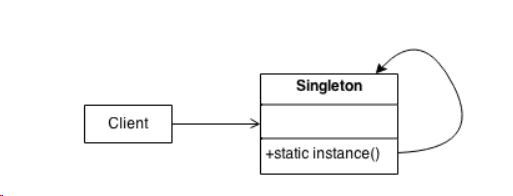
\includegraphics{GALLEYS/images/chapter1/diagram01}
\begin{multicols}{2}
\vspace{-20pt}
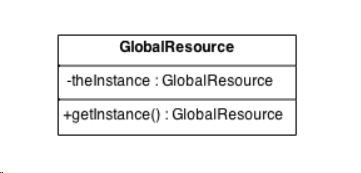
\includegraphics{GALLEYS/images/chapter1/diagram2}
\textbf{Mô tả đôi nét:} để đảm bảo chỉ có duy nhất một instance trong một class thì ta tạo ra một construct mang thuộc tính private.\\
Nhưng nó nảy sinh ra một vấn đề là private chỉ có thể được khai báo ở nội bộ của class đó.
\end{multicols}
Ta có thể vừa khắc phục vấn đề chỉ có một instance bằng phương thức public static(phương thức tĩnh) vì thành phần static chỉ có thể gọi một lần. Cụ thể :\\\\
- Lớp Singleton khai báo static method getInstance() trả về cùng một thể hiện của lớp riêng của nó.\\
- Constructor của Singleton phải là private. Gọi phương thức getInstance() là cách duy nhất để lấy đối tượng Singleton.
Chúng Ta sẽ đi sâu hơn vào ví dụ để tìm hiểu:\\
\begin{multicols}{2}
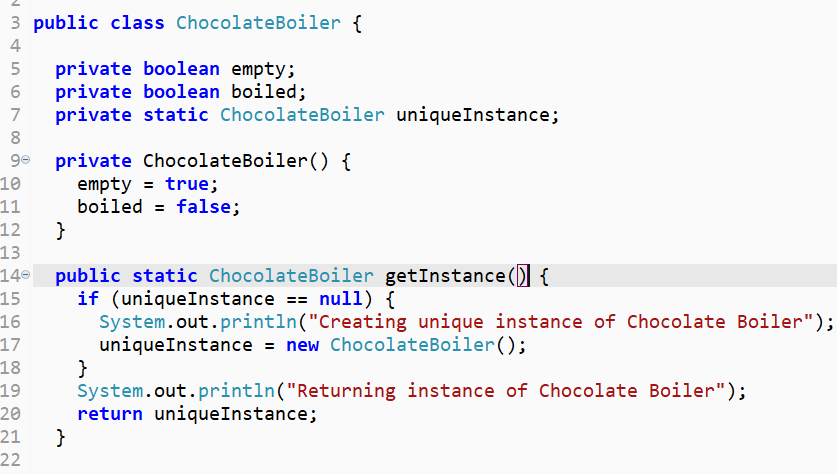
\includegraphics[height=0.23\textheight]{GALLEYS/images/chapter1/images1s}

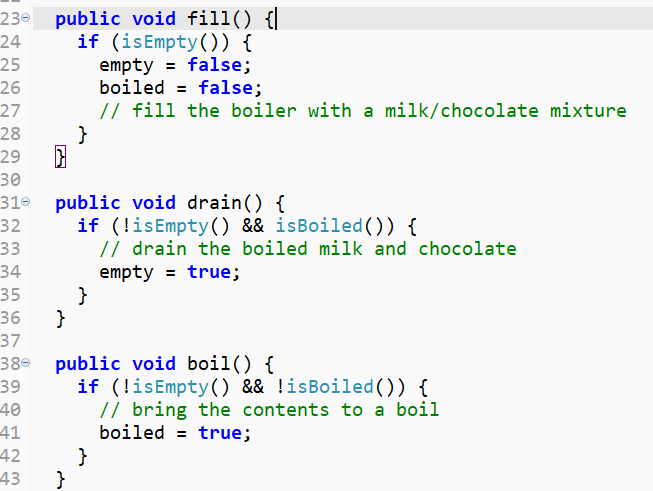
\includegraphics[height=0.25\textheight]{GALLEYS/images/chapter1/images1f}
\end{multicols}
+) trong ví dụ về nồi hơi chocolate ở trên:\\
Ta có một construct với phạm vi là private (private ChocolateBoiler()) và một đối tượng singleton sẽ không cần phải khởi tạo mà chỉ cần gọi đến phương thức tĩnh getInstance(). Đặc biệt việc khởi tạo đối tượng thông qua phương thức tĩnh getInstance() chỉ được thực hiện 1 lần.\\
Đây là kết quả:\\
\begin{center}
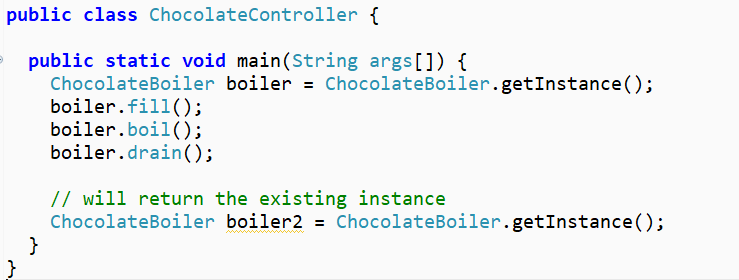
\includegraphics[scale=0.75]{GALLEYS/images/chapter1/images2}\\
\vspace{1cm}
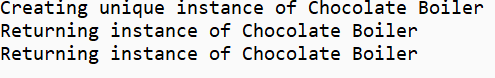
\includegraphics{GALLEYS/images/chapter1/images3}
\end{center}
Có thể thầy chỉ có duy nhất một đối tượng được khởi tạo trong lớp dù có khai báo bao nhiêu lần đi nữa.

\section{Singleton Pattern trong thực tế}
Dưới đây là một số trường hợp sử dụng của Singleton Pattern thường gặp:
\begin{itemize}
	\item	Vì class dùng Singleton chỉ tồn tại 1 Instance (thể hiện) nên nó thường được dùng cho các trường hợp giải quyết các bài toán cần truy cập vào các ứng dụng như: Shared resource, Logger, Configuration, Caching, Thread pool, …\\
	\item	Một số design pattern khác cũng sử dụng Singleton để triển khai: Abstract Factory, Builder, Prototype, Facade,…\\
	\item	Đã được sử dụng trong một số class của core java như: java.lang.Runtime, java.awt.Desktop.
\end{itemize}






\chapter{Observer Pattern}

\section{Định nghĩa}
Observer Pattern là một trong những Pattern thuộc nhóm hành vi (Behavior Pattern). Nó định nghĩa mối phụ thuộc một – nhiều giữa các đối tượng để khi mà một đối tượng có sự thay đổi trạng thái, tất các thành phần phụ thuộc của nó sẽ được thông báo và cập nhật một cách tự động.

\section{Mục đích sử dụng}
Mục đích và lợi ích:
\begin{itemize}
	\item	Dễ dàng mở rộng với ít sự thay đổi : mẫu này cho phép thay đổi Subject và Observer một cách độc lập. Chúng ta có thể tái sử dụng các Subject mà không cần tái sử dụng các Observer và ngược lại. Nó cho phép thêm Observer mà không sửa đổi Subject hoặc Observer khác. Vì vậy, nó đảm bảo nguyên tắc Open/Closed Principle (OCP).\\
	\item	Sự thay đổi trạng thái ở 1 đối tượng có thể được thông báo đến các đối tượng khác mà không phải giữ chúng liên kết quá chặt chẽ.\\
	\item	Một đối tượng có thể thông báo đến một số lượng không giới hạn các đối tượng khác.
\end{itemize}
Bên cạnh những lợi ích, chúng ta cần xem xét đến trường hợp cập nhật không mong muốn (Unexpected update) của Subject. Bởi vì các Observer không biết về sự hiện diện của nhau, nó có thể gây tốn nhiều chi phí của việc thay đổi Subject.
\section{Trường hợp cụ thể}
Observer Pattern được áp dụng khi:

\begin{itemize}
	\item Khi thay đổi một đối tượng, yêu cầu thay đổi đối tượng khác và chúng ta không biết có bao nhiêu đối tượng cần thay đổi, những đối tượng này là ai.\\
	\item Sử dụng trong ứng dụng broadcast-type communication.\\
	\item Sử dụng để quản lý sự kiện (Event management).\\
	\item Sử dụng trong mẫu mô hình MVC (Model View Controller Pattern) : trong MVC, mẫu này được sử dụng để tách Model khỏi View. View đại diện cho Observer và Model là đối tượng Observable.
\end{itemize}
\section{Mô hình câu trúc}
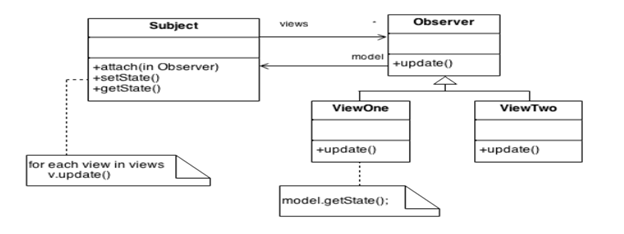
\includegraphics{GALLEYS/images/chapter2/diagram1}\\
\textbf{Subject} : cung cấp các phương thức để thêm, loại bỏ, thông báo observer.\\
\textbf{Observer} : định nghĩa một phương thức update() cho các đối tượng sẽ được subject thông báo đến khi có sự thay đổi trạng thái. \\
\textbf{ViewOne,ViewTwo ..} : có thể là bất cứ lớp con nào implement Observer interface. Mỗi observer đăng ký với một subject cụ thể để nhận được cập nhật.\\
Khi có một thay đổi nào đó, subject sẽ thông báo khi các observer có sự thay đổi. VD:
\begin{center}
	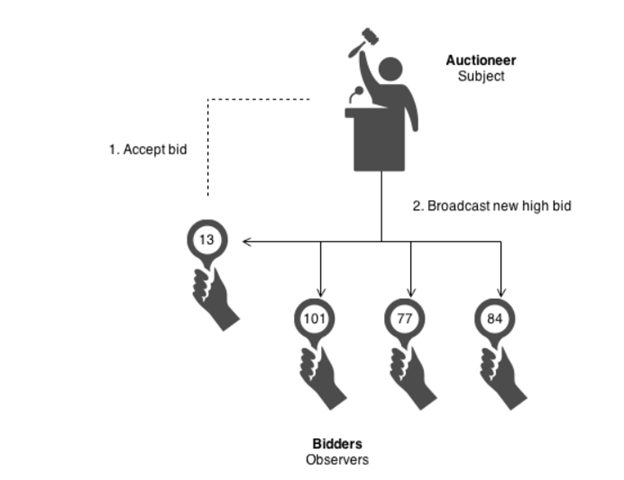
\includegraphics{GALLEYS/images/chapter2/exdiagram}\\
\end{center}
\hspace{0.5cm}Trong một cuộc đấu giá, khi một người tham gia giơ bảng giá lên,đấu giá viên bắt đầu quan sát , khi được chấp thuận, bảng giá mới sẽ được phát cho tất cả cấc nhà thầu tham gia khác.\\
   Để trực quan hơn chúng ta sẽ đến với phần ví dụ minh họa:\\
   Đây là một minh họa về trạm thời tiết Weather Station:\\

\begin{multicols}{2}
	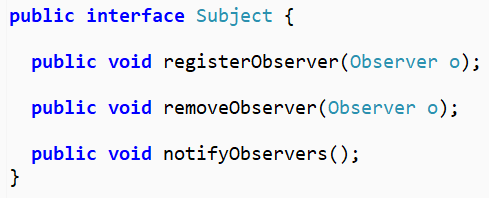
\includegraphics[width=1\columnwidth]{GALLEYS/images/chapter2/images1}\\\\\\
	Trong subject interfact có:\\
	+) public void registerObserver(Observer o) và public void removerObserver(Observer o) : cả 2 phương thức này lấy một Observer làm đối số, đó là Observer được remove hoặc register.\\
	+)phương thức notifyObservers() : phương thức này được gọi để thông báo các thành viên khi subject thay đổi.
\end{multicols}
	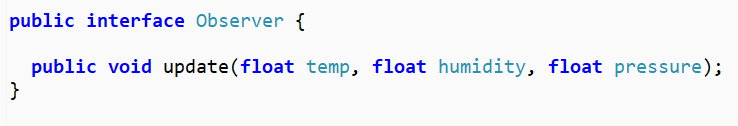
\includegraphics{GALLEYS/images/chapter2/images2}\\
	Giao diện observer được implement bởi tất cả các nhà quan sát, vì vậy tất cả phải thực hiện phương thức update() với đối số là các trạng thái mà observer nhận được khi subject đo thời tiết thay đổi.
\begin{multicols}{2}
	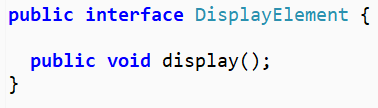
\includegraphics{GALLEYS/images/chapter2/images3}\\
	Đây là phần giao diện để hiển thị,chúng sẽ gọi phần tử hiển thị khi cần hiển thị.
\end{multicols}
\begin{multicols}{2}
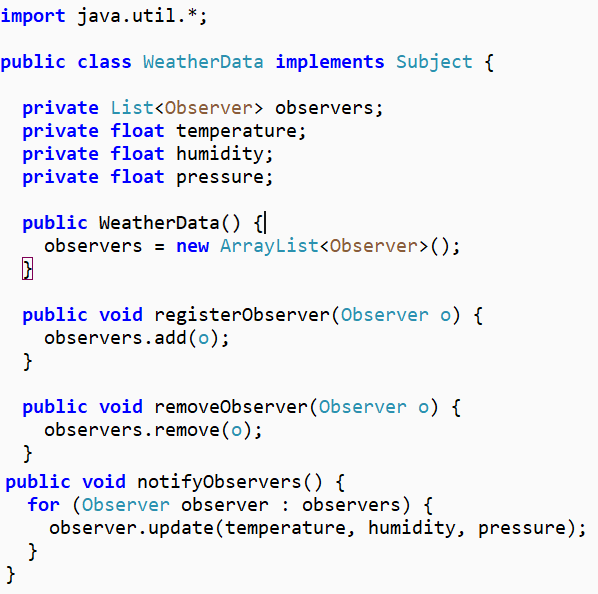
\includegraphics[width=\columnwidth]{GALLEYS/images/chapter2/images4}\\
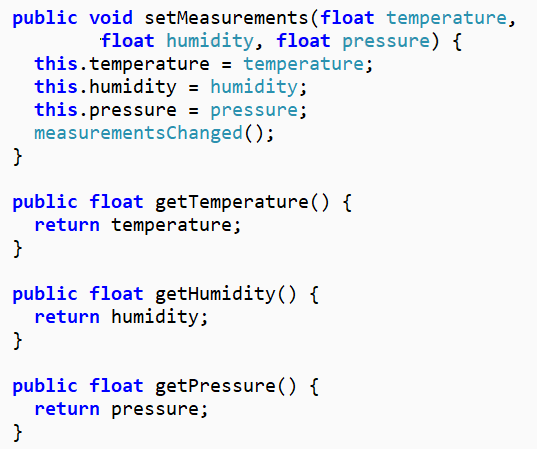
\includegraphics[width=\columnwidth]{GALLEYS/images/chapter2/images5}\\
\end{multicols}
Đây là phần chứa dữ liệu về thời tiết, lớp này được implement từ subject gồm:\\
+) có một ArrayList<Observer> (phạm vi private) dùng để lưu trữ các observer, nó được tạo ở trong construct.\\
+) các thuộc tính có bản như temperature (nhiệt độ), humidity(độ ẩm), pressure(áp suất) có phạm vi truy cập là private và kiểu dữ liệu float.\\
+) các phương thức registerObserver(Observer o) thêm các observer vào trong List khi muốn đăng ký
Phương thức removeObserver(Observer o) khi một observer muốn un-register nó sẽ xóa nó ra khỏi List\\
+) phương thức notifyObservers() sẽ thông báo update() trạng thái đến tất cả các observer\\
+) phương thức measurementsChanged() sẽ gọi đến notifyObservers() nhằm thông báo đến Observer khi có sự thay đổi phép đo.\\
+) phương thức setMeasurements() sẽ thay đổi giá trị phép đo và gọi đến measurementsChanged() nhằm thông báo đến các observers là giá trị đã thay đổi.\\
+) cuối cùng là các phương thức getTemperature() , getHumidity() và getPressure().\\
	Chúng ta sẽ đi đến phần màn hình hiển thị:\\
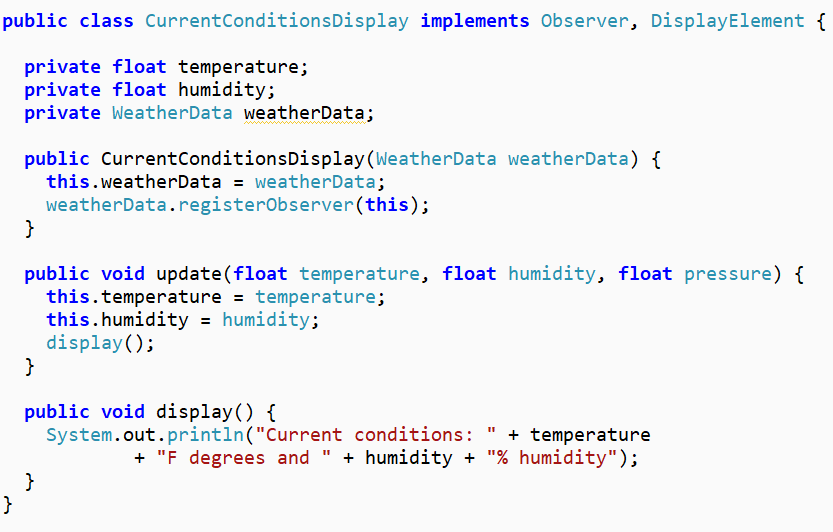
\includegraphics{GALLEYS/images/chapter2/images6}\\
Đây là màn hình thống kê và dự báo hiển thị cho nhiệt độ và độ ẩm, có một construct dùng để thông qua WeatherData và nó được dùng để đăng ký observer.
Phương thức update dùng để lưu nhiệt độ và áp suất đo được, từ đó đưa ra dự báo, khi có thay đổi . đặc biệt, WeatherData không được sử dụng, nhưng nó sẽ giúp cho việc hủy đăng ký với tư cách một observer.\\
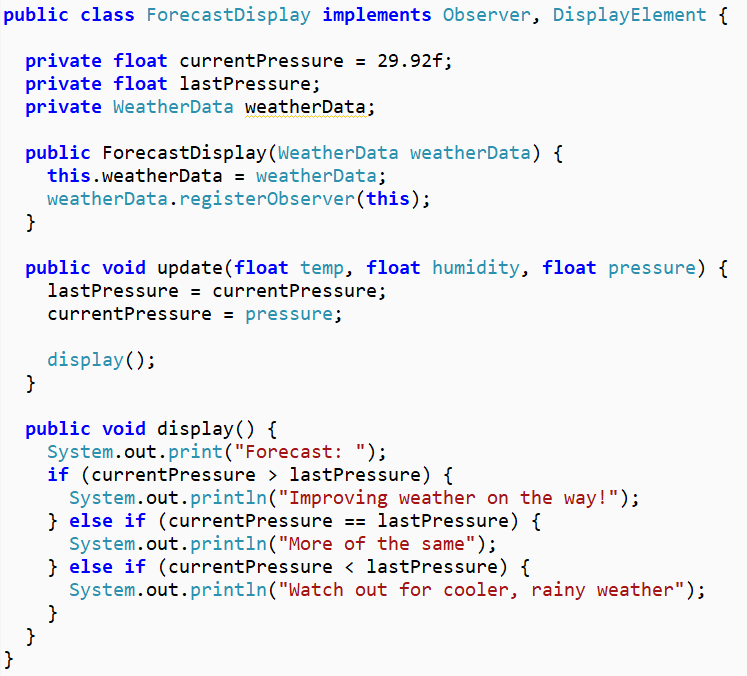
\includegraphics{GALLEYS/images/chapter2/images7}\\
Đây là màn hình thống kê và dự báo hiển thị cho áp suất chênh lệch. \\
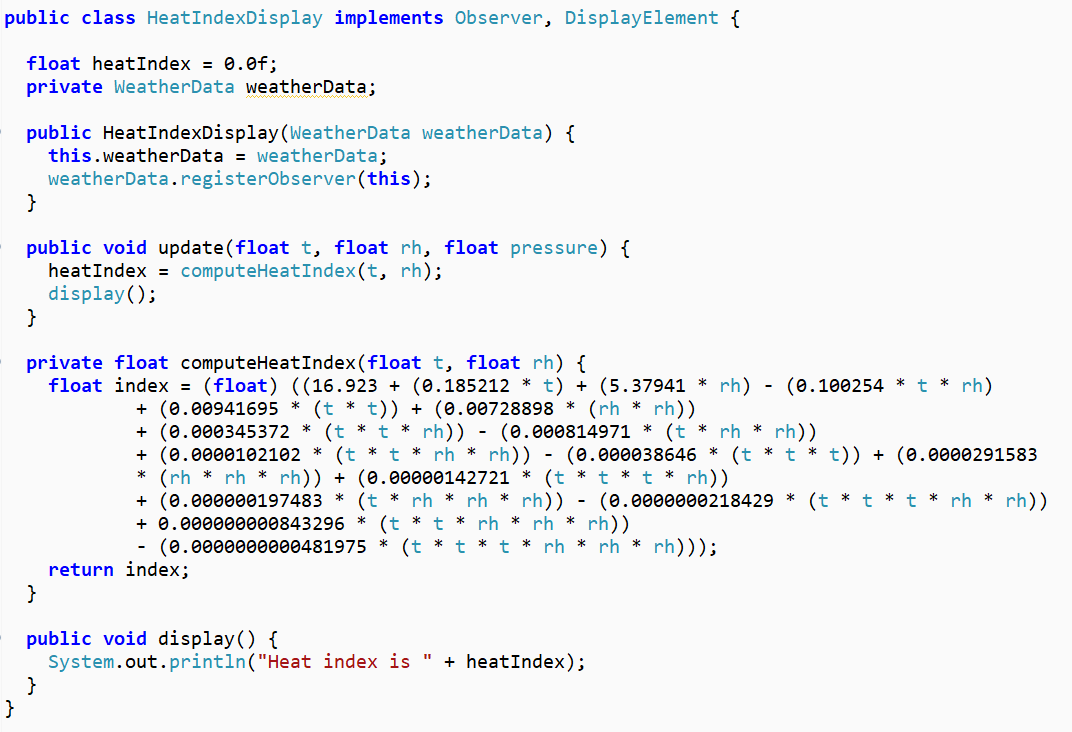
\includegraphics[width=\columnwidth,height=.45\textheight]{GALLEYS/images/chapter2/images8}\\
Đây là màn hình thống kê và dự báo hiển thị cho chỉ số nhiệt.\\\\
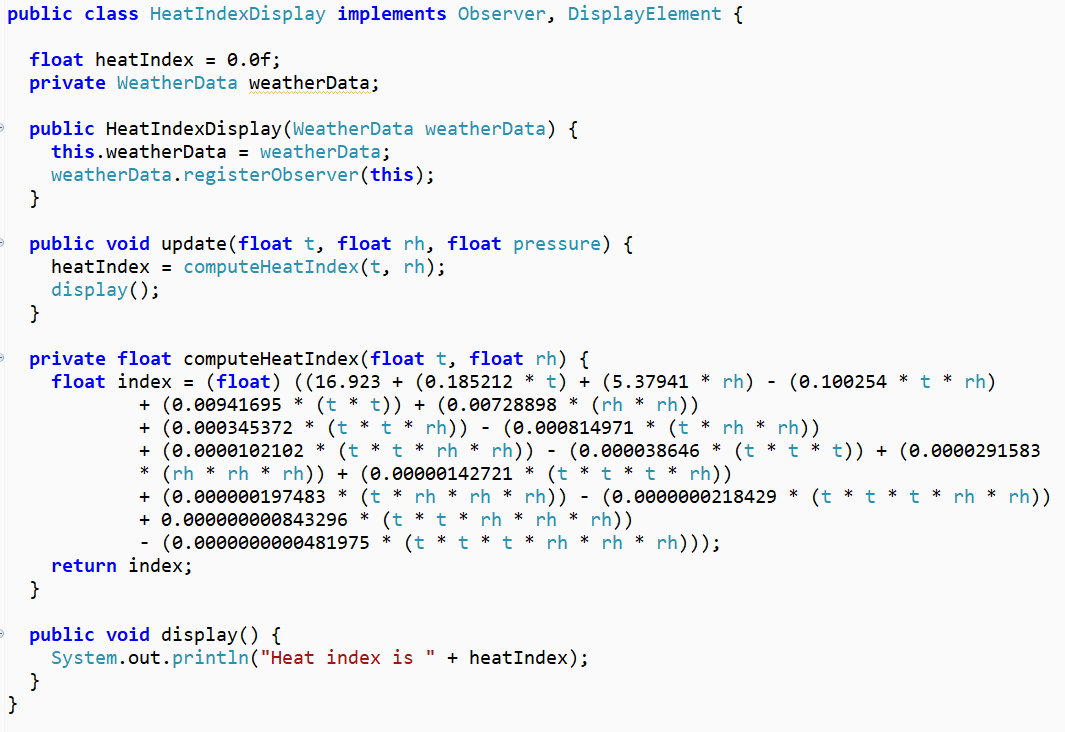
\includegraphics[width=\columnwidth,height=.5\textheight]{GALLEYS/images/chapter2/images9}\\
Đây là màn hình thống kê và dự báo hiển thị cho thống kê nhiệt độ.\\
Toàn bộ dữ liệu được thu thập từ trạm thời tiết\\
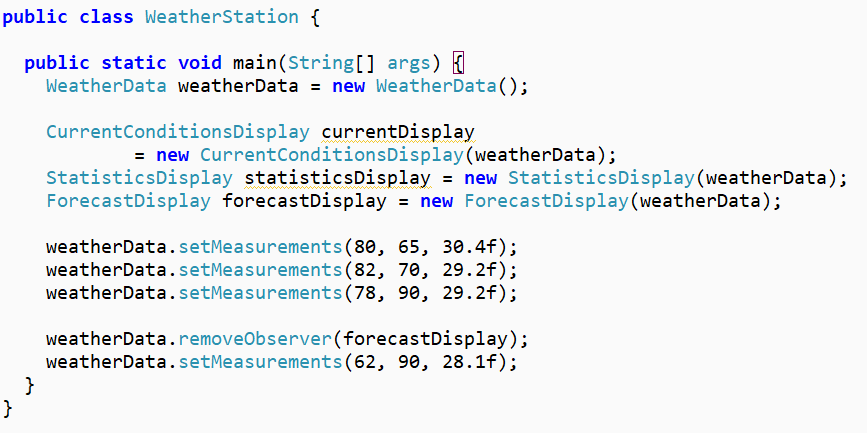
\includegraphics[width=\columnwidth,height=.4\textheight]{GALLEYS/images/chapter2/images10}\\
Trạm thời tiết sẽ hiển thi thông tin\\
Đây là kết quả:\\\\
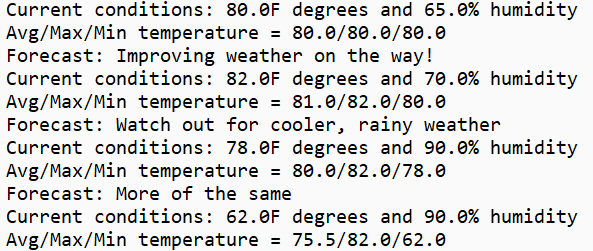
\includegraphics[width=\columnwidth,height=.3\textheight]{GALLEYS/images/chapter2/images11}\\\\
Mẫu thiết kế Observer (quan sát) có thể được sử dụng bất cứ khi nào mà một đối tượng có sự thay đổi trạng thái, tất các thành phần phụ thuộc của nó sẽ được thông báo và cập nhật một cách tự động.\\




\chapter{Iterator pattern}

\section{Định nghĩa}
Iterator Pattern là một trong những Pattern thuộc nhóm hành vi (Behavior Pattern). Nó được sử dụng để “Cung cấp một cách thức truy cập tuần tự tới các phần tử của một đối tượng tổng hợp, mà không cần phải tạo dựng riêng các phương pháp truy cập cho đối tượng tổng hợp này”.\\

Nói cách khác, một Iterator được thiết kế cho phép xử lý nhiều loại tập hợp khác nhau bằng cách truy cập những phần tử của tập hợp với cùng một phương pháp, cùng một cách thức định sẵn, mà không cần phải hiểu rõ về những chi tiết bên trong của những tập hợp này.

\section{Mục đích sử dụng}
Nếu trong project của các bạn có quá nhiều cấu trúc dạng danh sách như cấu trúc cây, mảng, ngăn xếp, hàng đợi.... Và bạn muốn có một quy tắc chung cho chúng như đều có thêm sửa xoá chẳng hạn. Như vậy lúc này chúng ta có thể tìm tới Iterator.
\section{Trường hợp cụ thể}
Iterator Pattern được áp dụng khi:

\begin{itemize}
	\item Cần truy cập nội dung của đối tượng trong tập hợp mà không cần biết nội dung cài đặt bên trong nó.\\
	\item Hỗ trợ truy xuất nhiều loại tập hợp khác nhau.\\
	\item Cung cấp một interface duy nhất để duyệt qua các phần tử của một tập hợp.\\
\end{itemize}
\section{Mô hình câu trúc}
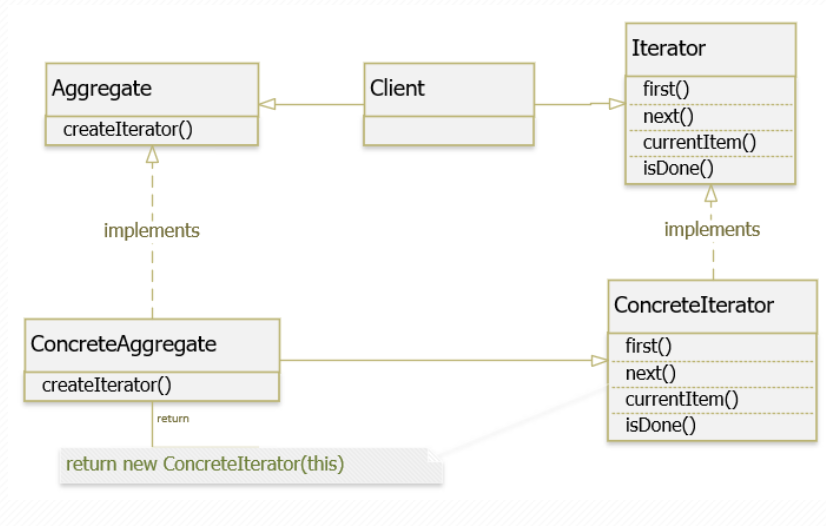
\includegraphics[width=\columnwidth]{GALLEYS/images/chapter3/diagram1}\\
\textbf{Aggregate} : là một interface định nghĩa định nghĩa các phương thức để tạo Iterator object.\\
\textbf{ConcreteAggregate} : cài đặt các phương thức của Aggregate, nó cài đặt interface tạo Iterator để trả về một thể hiện của ConcreteIterator thích hợp. \\
\textbf{Iterator} :  là một interface hay abstract class, định nghĩa các phương thức để truy cập và duyệt qua các phần tử. \\
\textbf{ConcreteIterator} :  cài đặt các phương thức của Iterator, giữ index khi duyệt qua các phần tử. \\
\textbf{Client} : đối tượng sử dụng Iterator Pattern, nó yêu cầu một iterator từ một đối tượng collection để duyệt qua các phần tử mà nó giữ. Các phương thức của iterator được sử dụng để truy xuất các phần tử từ collection theo một trình tự thích hợp.\\\\
VD cụ thể:\\
Tình huống: mô tả thực đơn cho những bữa ăn của hai cửa hàng có PancakeHouseMenu và DinnerMenu. Nhưng hai menu này được thực hiện khá là khác nhau
\newpage
\begin{multicols}{2}
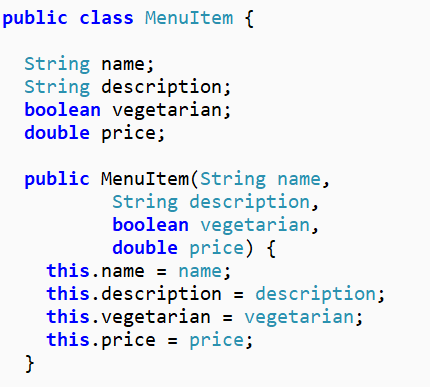
\includegraphics[width=1\columnwidth]{GALLEYS/images/chapter3/images1}\\
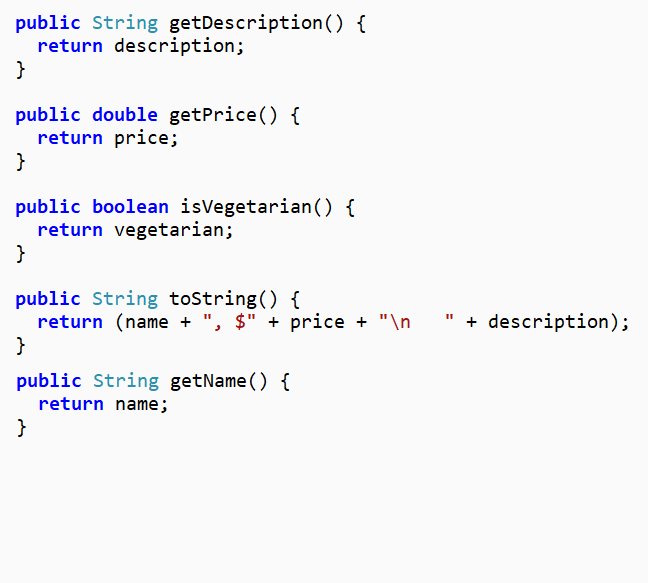
\includegraphics[width=1\columnwidth]{GALLEYS/images/chapter3/images2}
\end{multicols}
Trong class này chúng ta có những hàm cơ bản:\\
Hàm construct khởi tạo name,description,vegetarian,price
Các thuộc tính\\ name(String),description(String),vegetarian(boolean),price(double) các thuộc tính này đều có phạm vi là private.
Các hàm getter và setter cho các trường giá trị.\\

	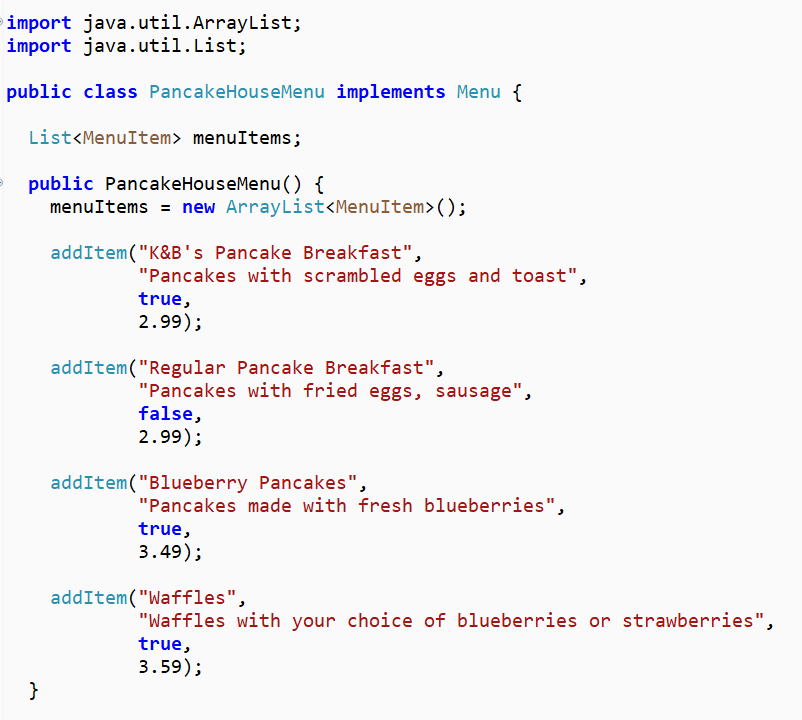
\includegraphics[width=1\columnwidth,height=0.51\textheight]{GALLEYS/images/chapter3/images3}\\
	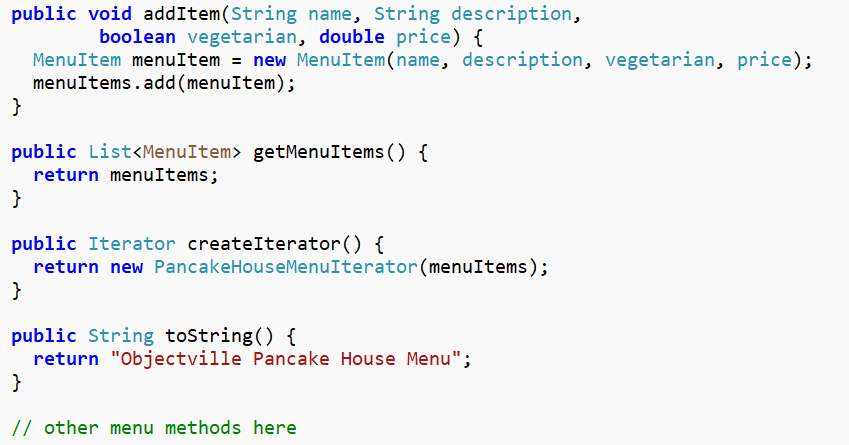
\includegraphics[width=1\columnwidth,height=0.48\textheight]{GALLEYS/images/chapter3/images4}\\\\
Tại PancakeHouseMenu:\\
- Có ArrayList<> dùng để lưu trữ dữ liệu.\\
- Trong construct của lớp mỗi menu item được thêm vào ArrayList<>, mỗi menuItem có tên, mô tả, đồ ăn chay hay không và giá tiền.\\
- Phương thức addItem() dùng để thêm menu mới vào trong ArrayList<>,
Phương thức getMenuItem dùng để trả về danh sách các menu.\\
- Phương thức createIterator() cho phép chúng ta trả về danh sách menu theo iterator pattern mà chúng ta sẽ nói rõ hơn nữa ở phía sau.\\

\begin{center}
	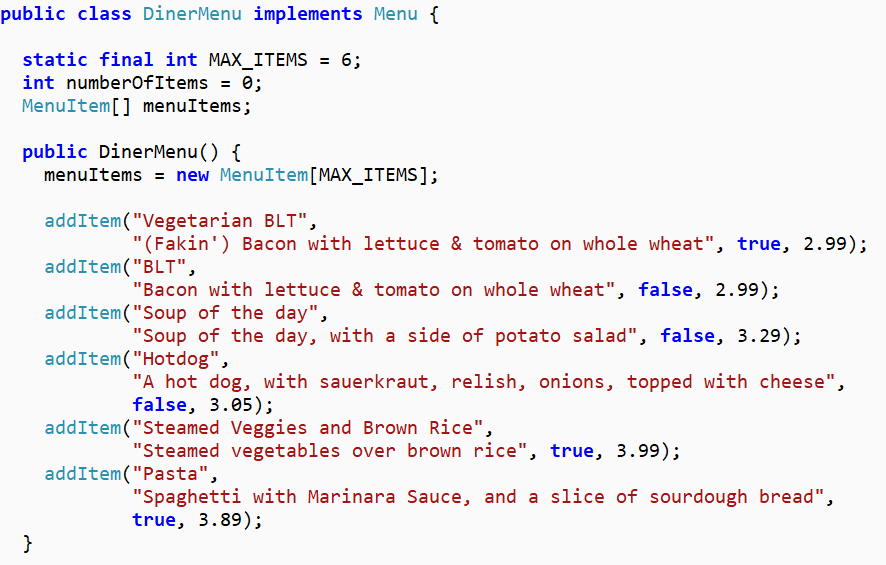
\includegraphics[width=1\columnwidth,height=0.48\textheight]{GALLEYS/images/chapter3/images5}\\
	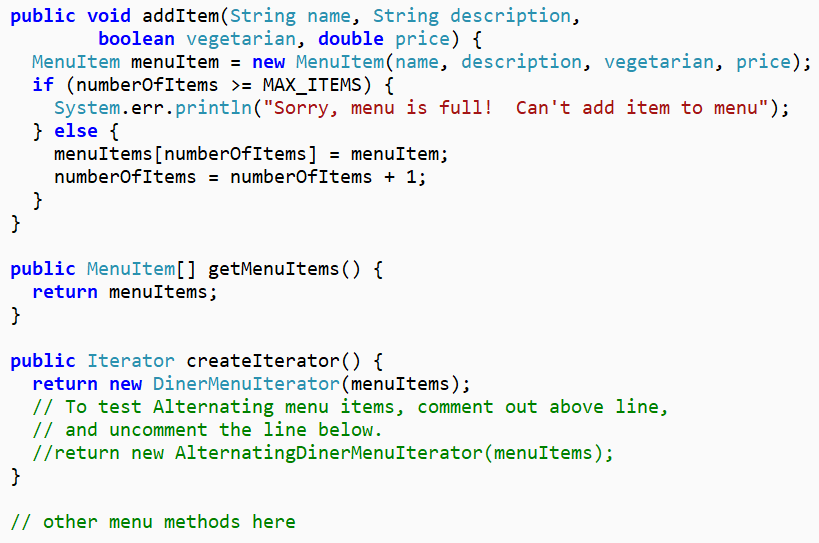
\includegraphics[width=1\columnwidth,height=0.48\textheight]{GALLEYS/images/chapter3/images6}\\
\end{center}
Trong DinnerMenu có cách thức hơi khác so với PancakeHouseMenu:\\
- Trong class này sử dụng Array thay cho ArrayList<> nhằm mục đích quản lí số lượng các menu, và lấy menu một cách đơn giản hơn.\\
- Phương thức addItem() sẽ kiểm tra nếu số lượng thực đơn đã đầy, item đó sẽ không được thêm vào mảng.\\
- Phương thức createIterator() có tác dụng tương tự như trong class PancakeHouseMenu. Đặc biệt cách thức này chúng ta sẽ chỉ biết là nó return về menuItem mà không biết nó được triển khai như thế nào.\\

 Những phương thức khác đều hoạt động tương tự như PancakeHoueMenu.Nhưng một vấn đề nảy ra: nếu muốn in ra menuItem của 2 menu này cho một nữ phục vụ (Waitress) sẽ rất là khó khăn vì cú pháp của array và arrayList khác nhau, và cữ mỗi menu thực hiện in một lần cũng mất thời gian hay là việc phân loại bữa trưa và bữa chiều của 2 menu và in ra thực đơn bữa trưa (chiều). vì thế chúng ta cần phải cho chúng implements menu chung để giảm thiểu các vòng lặp.\\
Class menu sẽ giải quyết điều đó: \\
\begin{multicols}{2}
	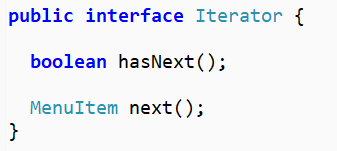
\includegraphics[width=1\columnwidth]{GALLEYS/images/chapter3/images7}
	Trong interface Iterator, có 2 phương thức gói gọn là hasNext() cho chúng ta biết có còn phần tử để duyệt qua hay không và next() trả về đối tượng tiếp theo trong tập hợp
\end{multicols}
\begin{multicols}{2}
	Giao diện interface Menu tạo ra phương thức createIterator().\\
	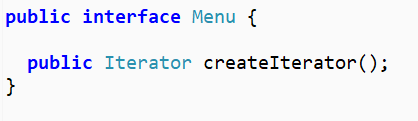
\includegraphics[width=1\columnwidth]{GALLEYS/images/chapter3/images8}
\end{multicols}
\begin{center}
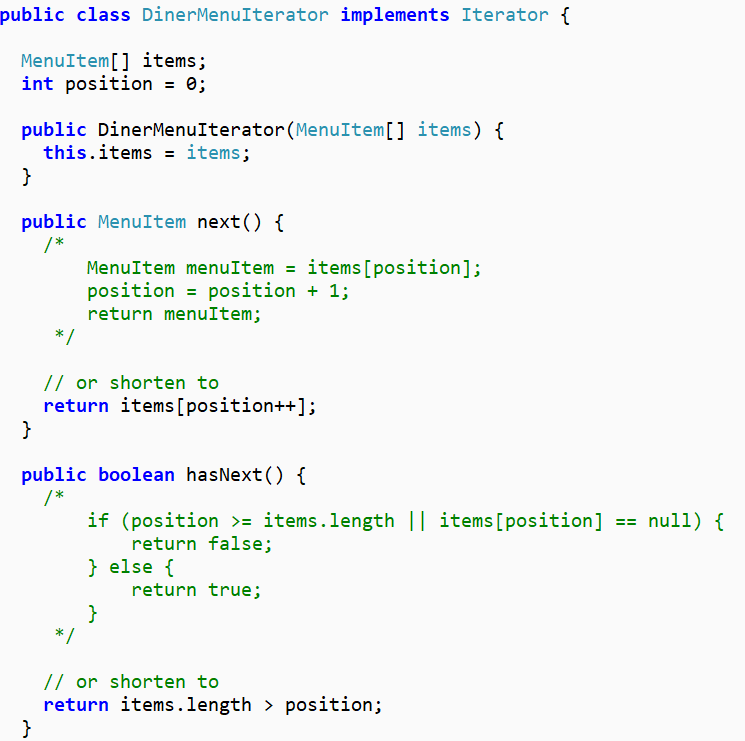
\includegraphics{GALLEYS/images/chapter3/images9}\\
\end{center}
Class này được implement từ interface Iterator.\\
Với một position dùng để duy trì vị trí lặp trên mảng . mặc định bằng 0.\\
Hàm construct lấy mảng mà chúng duyệt qua.\\
Việc cho các menu implement một interface iterator đã giúp giảm bớt độ phức tạp dành cho nữ phục vụ. \\
\begin{center}
	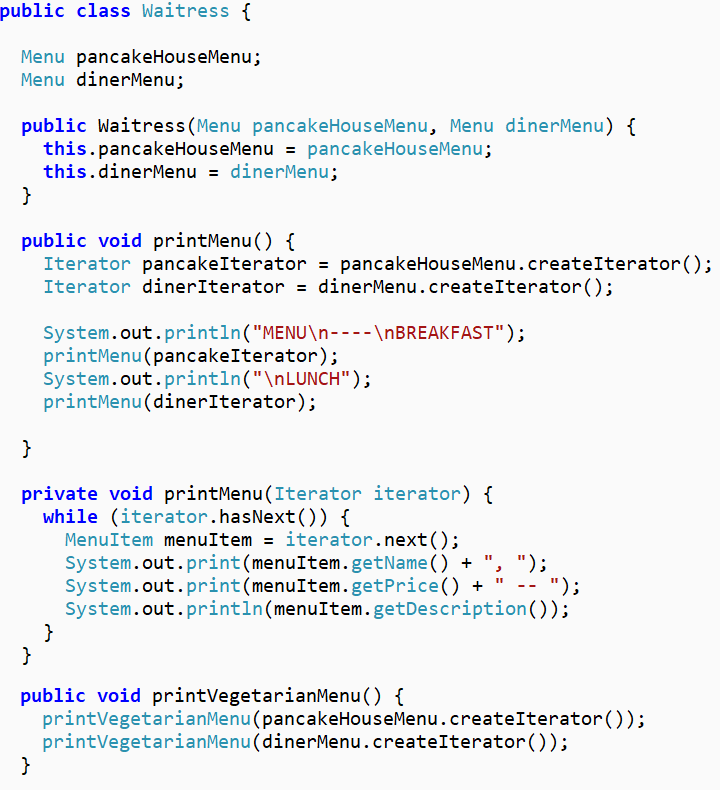
\includegraphics[width=1\columnwidth,height=0.7\textheight]{GALLEYS/images/chapter3/images10}\\
\end{center}
 Trong hàm khởi tạo của Waitress sẽ khởi tạo ra 2 menu.\\
Phương thức printMenu khởi tạo 2 Iterator.\\
Sau đó printMenu được overload với mỗi iterator.\\
Phương thức private printMenu in ra danh sách menu.\\
\begin{center}
	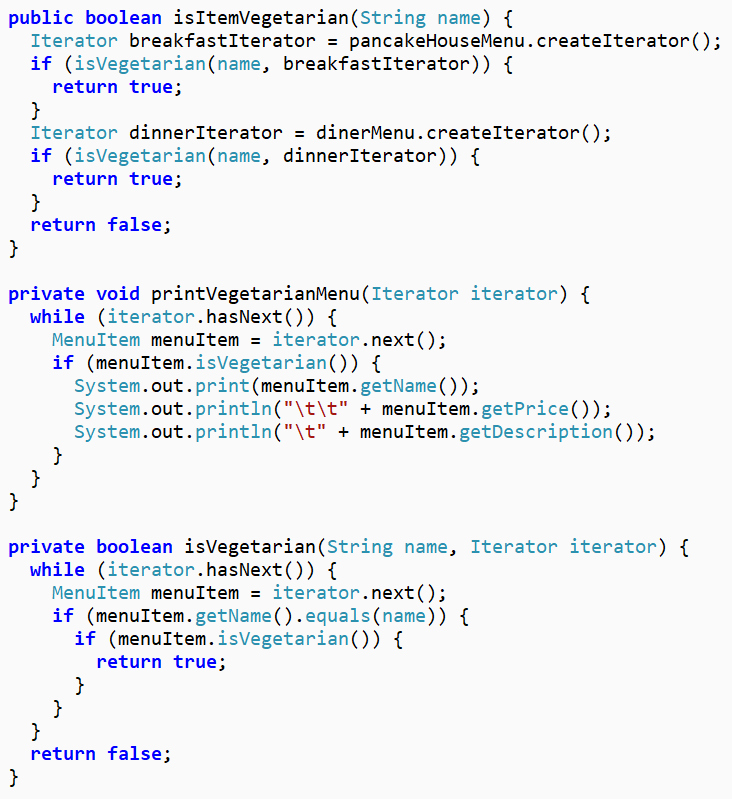
\includegraphics[width=1\columnwidth,height=0.7\textheight]{GALLEYS/images/chapter3/images11}\\
\end{center}
Tương tự chúng ta sẽ triển khai được các lớp khác.\\
Và đây là kết quả:
\begin{center}
	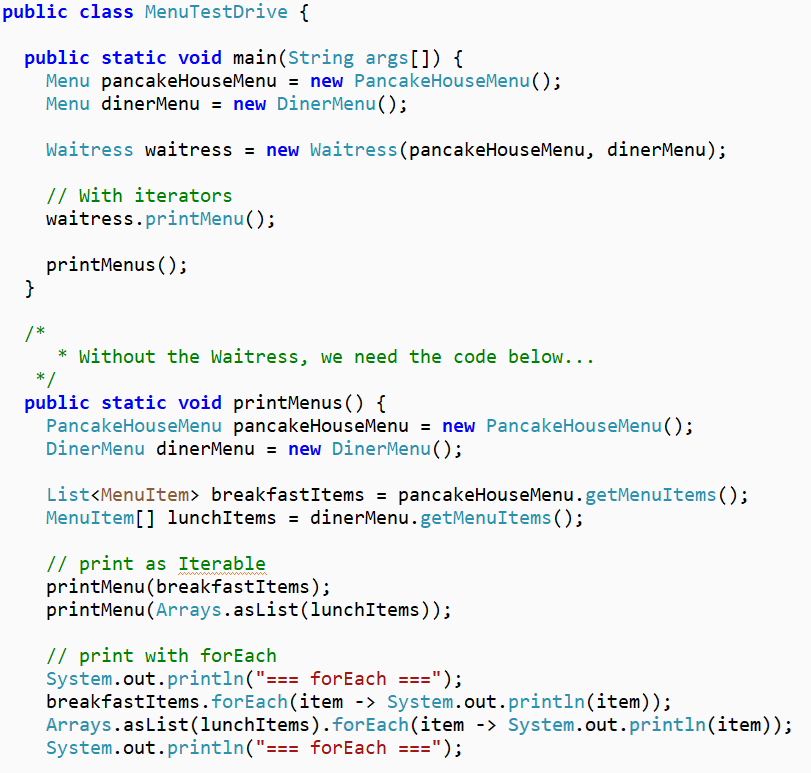
\includegraphics[width=1\columnwidth,height=0.4\textheight]{GALLEYS/images/chapter3/images12}\\
	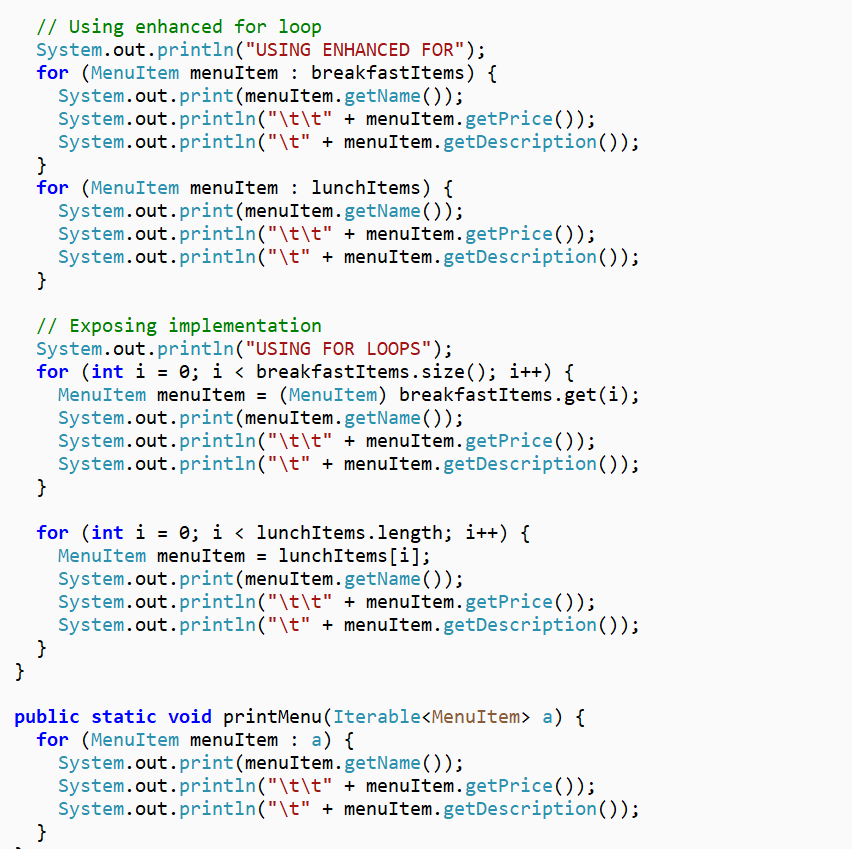
\includegraphics[width=1\columnwidth,height=0.5\textheight]{GALLEYS/images/chapter3/images13}\\
\end{center}
\begin{center}
	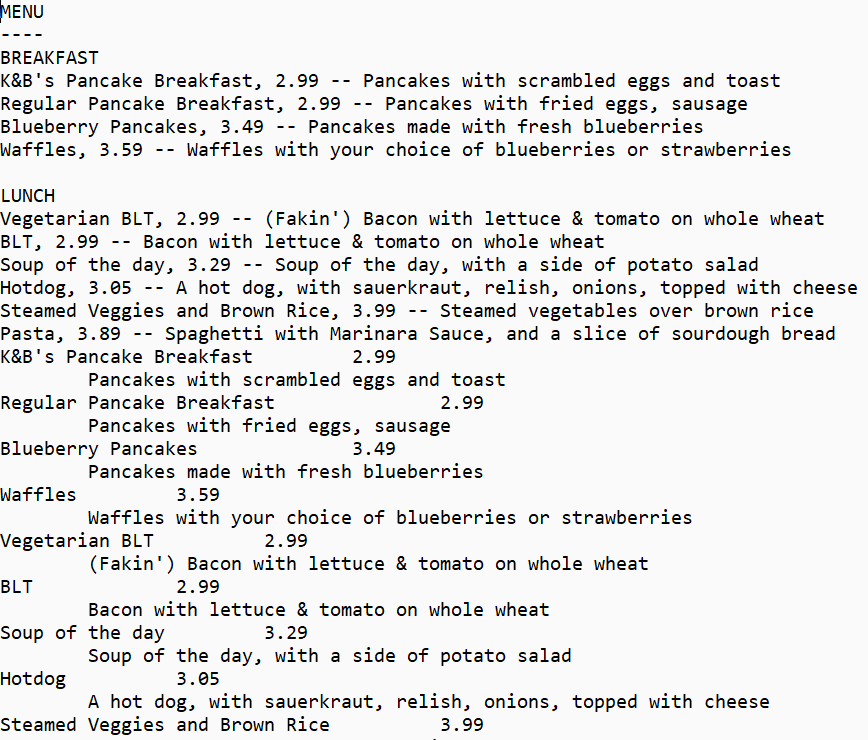
\includegraphics[width=1\columnwidth,height=0.8\textheight]{GALLEYS/images/chapter3/images14}\\
\end{center}
Đây là một phần của kết quả.\\
Như vậy Iterator pattern giúp chúng ta in ra danh sách các phần tử một cách rất đơn giản, nó là một trong những pattern được ứng dụng khá cao trong thực tế.

\chapter{Decorator Pattern}

\section{Định nghĩa}
Decorator pattern là một trong những Pattern thuộc nhóm cấu trúc (Structural Pattern). Nó cho phép người dùng thêm chức năng mới vào đối tượng hiện tại mà không muốn ảnh hưởng đến các đối tượng khác. Kiểu thiết kế này có cấu trúc hoạt động như một lớp bao bọc (wrap) cho lớp hiện có. Mỗi khi cần thêm tính năng mới, đối tượng hiện có được wrap trong một đối tượng mới (decorator class).\\

Decorator pattern sử dụng composition thay vì inheritance (thừa kế) để mở rộng đối tượng. Decorator pattern còn được gọi là Wrapper hay Smart Proxy.

\section{Mục đích sử dụng}
Mục đích và lợi ích:
\begin{itemize}
	\item Tăng cường khả năng mở rộng của đối tượng, bởi vì những thay đổi được thực hiện bằng cách implement trên các lớp mới.
	\item Client sẽ không nhận thấy sự khác biệt khi bạn đưa cho nó một wrapper thay vì đối tượng gốc.
	\item Một đối tượng có thể được bao bọc bởi nhiều wrapper cùng một lúc.
	\item Cho phép thêm hoặc xóa tính năng của một đối tượng lúc thực thi (run-time).
\end{itemize}

\section{Mô hình cấu trúc}
\begin{center}
	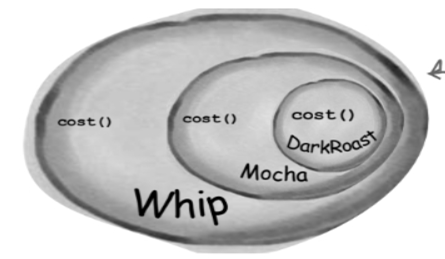
\includegraphics{GALLEYS/images/chapter4/diagram1}\\
\end{center}
\begin{center}
	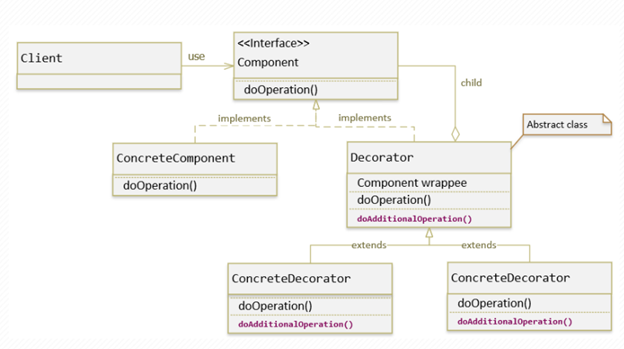
\includegraphics{GALLEYS/images/chapter4/diagram2}\\
\end{center}
Các thành phần trong mẫu thiết kế Decorator:\\
\textbf{Component} : là một interface quy định các method chung cần phải có cho tất cả các thành phần tham gia vào mẫu này.\\
\textbf{ConcreteComponent } : là lớp hiện thực (implements) các phương thức của Component.\\
\textbf{Decorator} : là một abstract class dùng để duy trì một tham chiếu của đối tượng Component và đồng thời cài đặt các phương thức của Component  interface.\\
\textbf{ConcreteDecorator } : là lớp hiện thực (implements) các phương thức của Decorator, nó cài đặt thêm các tính năng mới cho Component.\\
\textbf{Client} : đối tượng sử dụng Component.\\
VD:\\

Tình huống đặt ra trong quán cafee Starbuzz, giúp quản lí các loại đồ uống.\\
Khởi đầu là một lớp đồ uống :\\
\begin{multicols}{2}
	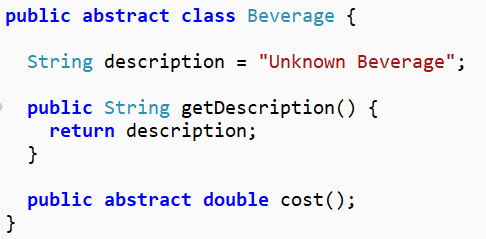
\includegraphics[width=1\columnwidth]{GALLEYS/images/chapter4/images1}\\
	
	Beverage là một lớp trừu tượng với một biến String description và hai phương thức trừu tượng getDescription() lấy ra thông tin đồ uống và cost() lấy ra giá của đồ uống.\\
	
	Lớp Beverage khá là đơn giản, nhưng đây là lớp cha của tất cả các lớp đồ uống – mọi lớp con đều phải extends từ đây.
	
\end{multicols}
\begin{center}
	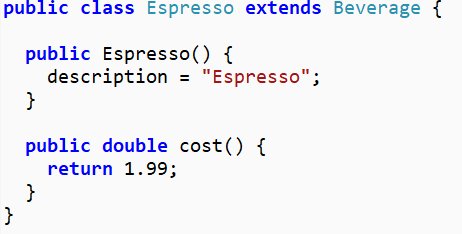
\includegraphics{GALLEYS/images/chapter4/images3}
\end{center}
Lớp cà phê Espresso có một construct khởi tạo thông tin là tên của loại cafee này và giá tiền là 1.99. 
Chúng ta sẽ tìm hiểu thêm một số loại sản phẩm khác:
\begin{multicols}{2}
	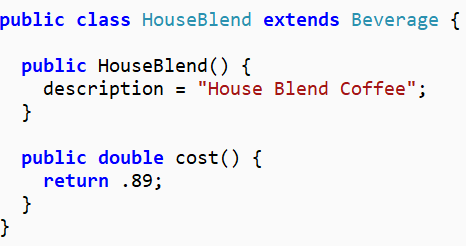
\includegraphics[width=0.9\columnwidth]{GALLEYS/images/chapter4/images4}
	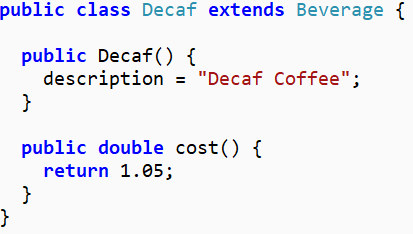
\includegraphics[width=0.9\columnwidth]{GALLEYS/images/chapter4/images5}
\end{multicols}
\begin{center}
	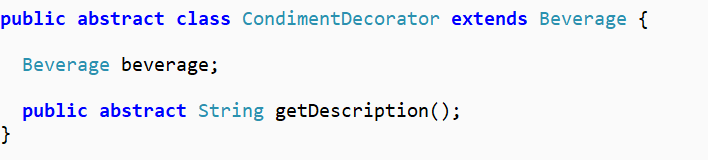
\includegraphics{GALLEYS/images/chapter4/images2}
\end{center}
Đây là lớp gia vị, nó phải kế thừa từ lớp đồ uống, ở đây có một phương thức trừu tượng getDescription() mô tả thông tin của gia vị.\\
Ở đây có 1 biến beverage và một lớp trừu tượng getDescription().
Nếu muốn một đồ uống nào đó có thêm gia vị , lớp đồ uống đó sẽ cần extends lại lớp này.

Như vậy có vẻ các lớp cơ sở khá là đầy đủ, chúng ta sẽ tiến hành đi sâu hơn vào các lớp con của chúng:\\
Lớp Espresso:\\

\begin{multicols}{2}
	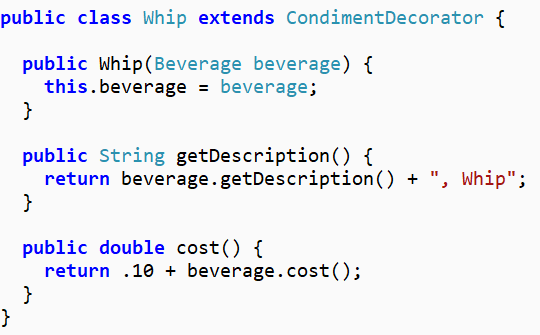
\includegraphics[width=0.9\columnwidth]{GALLEYS/images/chapter4/images6}
	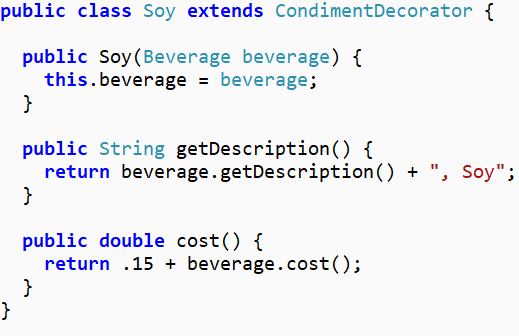
\includegraphics[width=0.9\columnwidth]{GALLEYS/images/chapter4/images7}
\end{multicols}

Điều thú vị ở đây là lớp nước uống có thêm gia vị này giá tiền sẽ được cộng thêm với giá cơ sở cho nước đó. Nó giảm độ phức tạp tính toán của nhà hàng.\\
Và đây là kết quả:
\begin{center}
	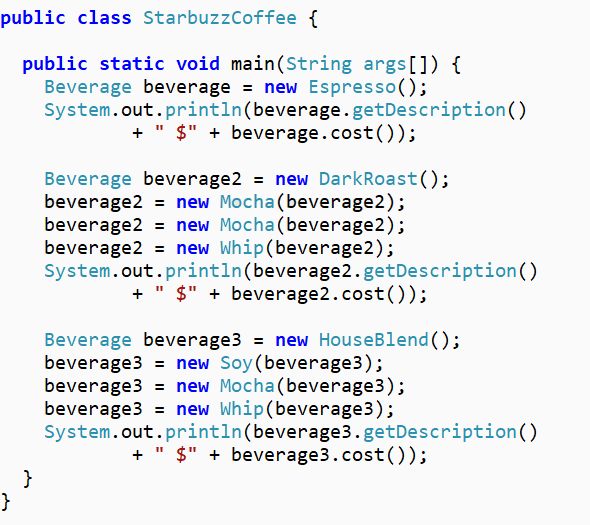
\includegraphics{GALLEYS/images/chapter4/images8}
	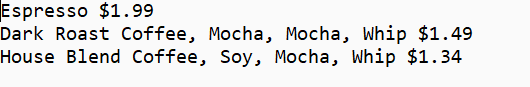
\includegraphics{GALLEYS/images/chapter4/images9}
\end{center}tế

\section{Decorator Pattern trong thực tế}
Decorator Pattern được áp dụng khi:

\begin{itemize}
	\item Khi muốn thêm tính năng mới cho các đối tượng mà không ảnh hưởng đến các đối tượng này.
	\item Khi không thể mở rộng một đối tượng bằng cách thừa kế (inheritance). Chẳng hạn, một class sử dụng từ khóa final, muốn mở rộng class này chỉ còn cách duy nhất là sử dụng decorator.
	\item Trong một số nhiều trường hợp mà việc sử dụng kế thừa sẽ mất nhiều công sức trong việc viết code. Ví dụ trên là một trong những trường hợp như vậy.
\end{itemize}


\chapter{Factory Pattern }
\section{Factory Pattern – Factory method}
\subsection{Định nghĩa}

Factory Method Design Pattern hay gọi ngắn gọn là Factory Pattern là một trong những Pattern thuộc nhóm Creational Design Pattern. Factory Pattern xác định một interface để tạo một đối tượng, nhưng cho phép các lớp con quyết định lớp nào sẽ khởi tạo.  Factory Pattern giao việc khởi tạo một đối tượng cụ thể cho lớp con.

Factory Pattern đúng nghĩa là một nhà máy, và nhà máy này sẽ “sản xuất” các đối tượng theo yêu cầu của chúng ta.

\subsection{Mục đích sử dụng}
Mục đích và lợi ích:
\begin{itemize}
\item	Factory Pattern giúp giảm sự phụ thuộc giữa các module (loose coupling): cung cấp 1 hướng tiếp cận với Interface thay thì các implement. Giúp chuơng trình độc lập với những lớp cụ thể mà chúng ta cần tạo 1 đối tượng, code ở phía client không bị ảnh hưởng khi thay đổi logic ở factory hay sub class.
\item Mở rộng code dễ dàng hơn: khi cần mở rộng, chỉ việc tạo ra sub class và implement thêm vào factory method.
\item Khởi tạo các Objects mà che giấu đi xử lí logic của việc khởi tạo đấy. Người dùng không biết logic thực sực được khởi tạo bên dưới phương thức factory.
\item Dễ dạng quản lý life cycle của các Object được tạo bởi Factory Pattern.
\item Thống nhất về naming convention: giúp cho các developer có thể hiểu về cấu trúc source code.
\end{itemize}

\subsection{Trường hợp cụ thể}
Factory Pattern được sử dụng khi:

\begin{itemize}
	\item Chúng ta có một super class với nhiều class con và dựa trên đầu vào, chúng ta cần trả về một class con. Mô hình này giúp chúng ta đưa trách nhiệm của việc khởi tạo một lớp từ phía người dùng (client) sang lớp Factory.
	\item Chúng ta không biết sau này sẽ cần đến những lớp con nào nữa. Khi cần mở rộng, hãy tạo ra sub class và implement thêm vào factory method cho việc khởi tạo sub class này.\\
Bạn có thể thấy Factory Pattern được áp dụng trong:
\item JDK: java.util.Calendar, ResourceBundle, NumberFormat, …
\item BeanFactory trong Spring Framework.
\item SessionFactory trong Hibernate Framework.
\end{itemize}
Bạn có thể thấy Factory Pattern được áp dụng trong:
\begin{itemize}
	\item JDK: java.util.Calendar, ResourceBundle, NumberFormat, …
	\item BeanFactory trong Spring Framework.
	\item SessionFactory trong Hibernate Framework.
\end{itemize}
\subsection{Mô hình câu trúc}
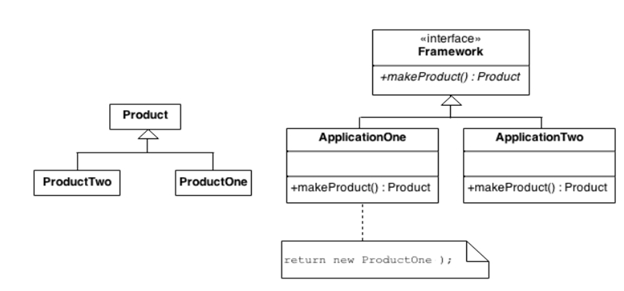
\includegraphics{GALLEYS/images/chapter5/diagram1}\\
\textbf{mô tả mô hình} : Product là obj cần phải khởi tạo, Framework là factory và Application là nơi quyết định xem đối tượng nào khởi tạo.\\
VD:\\
Giả sử trong một của hàng pizza, khách hàng muốn order 1 loại pizza, chúng có nhiểu loại, chúng ta xé quản lí những loại pizza đó một cách hợp lí. Hãy quan sát đoạn code để làm rõ vấn đề hơn, nhưng có một vấn đề là mỗi một vùng miền lại có một kiểu Pizza khác nhau,thương mại khác nhau. Cùng quan sát vấn đề:\\

Trong facory method những vấn đề liên quan đến tạo đối tượng sẽ được tạo một lớp riêng, cụ thể là một lớp trừu tượng.\\

\begin{center}
	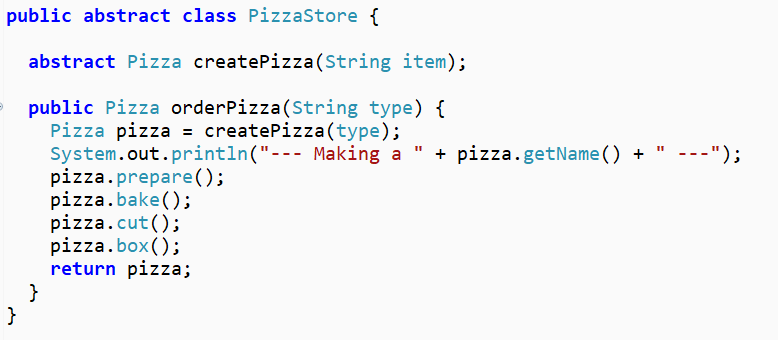
\includegraphics[width=1\columnwidth]{GALLEYS/images/chapter5/images1}
\end{center}
Đây là class PizzaStore :\\

Phương thức abstract createPizza() với phạm vi là protected dùng để xử lí việc tạo đối tượng và gói nó trong một lớp con. Điều này tách client code ra khỏi code tạo object dưới subclass.\\

Trong phương thức public orderPizza() sẽ có một biến Pizza để khởi tạo chiếc bánh mà khách hàng muốn đặt.\\

Các phương thức prepare(),bake(),cut(),box() thuộc về lớp pizza, nó là các thay đổi trên chiếc bánh.\\

Mỗi cửa hàng pizza ở mỗi vùng miền cũng khác nhau. Chúng sẽ được kế thừa từ lớp cơ sở PizzaStore.\\

\begin{center}
	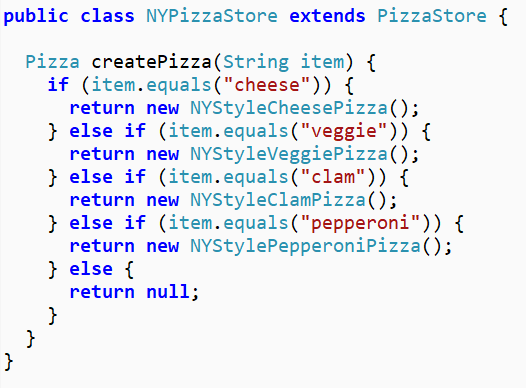
\includegraphics{GALLEYS/images/chapter5/images2}
\end{center}
Đây là một cửa hàng pizza NY\\
\begin{center}
	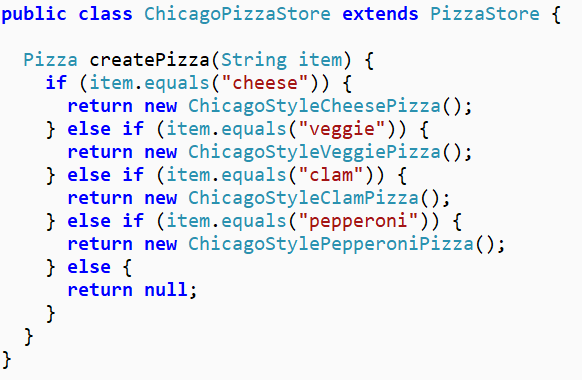
\includegraphics{GALLEYS/images/chapter5/images3}
\end{center}
\newpage
\begin{multicols}{2}
	\includegraphics[width=1\columnwidth]{GALLEYS/images/chapter5/images4}
	\includegraphics[width=1\columnwidth]{GALLEYS/images/chapter5/images5}
\end{multicols}

Lớp pizza này gồm các topping đi kèm của chiếc bánh.\\
Mỗi pizza có một loại tên(name), một loại bootk(dough), một loại nước sauce, và những loại topping đi kèm riêng biệt.\\

Ở đây chúng ta sử dụng StringBuffer để in ra thông tin của chiếc bánh đó.
mỗi pizza của mỗi vùng miền cụ thể có thể có cách làm khác nhau, chúng sẽ được kế thừa từ lớp Pizza.

\begin{multicols}{2}
	\includegraphics[width=1\columnwidth]{GALLEYS/images/chapter5/images6}
	\includegraphics[width=1\columnwidth]{GALLEYS/images/chapter5/images7}
\end{multicols}
Nhận xét: ở đây chúng ta có thể thấy đoạn code này phân thành 2 class với nhiệm vụ rõ ràng, đó là Product Classes có nhiệm vụ phát triển chiếc bánh và Creator Classes với nhiệm vụ createPizza() quyết định xem chiếc bánh pizza được phát triển như thế nào .\\
Đây là kết quả:

\begin{center}
	\includegraphics[height=.55\textheight]{GALLEYS/images/chapter5/images8}
	\includegraphics[height=.4\textheight]{GALLEYS/images/chapter5/images9}
\end{center}

\section{Factory Pattern – Abstract Factory method}
\subsection{Định nghĩa}

Abstract Factory pattern là một trong những Creational pattern. Nó là phương pháp tạo ra một Super-factory dùng để tạo ra các Factory khác. Hay còn được gọi là Factory của các Factory. Abstract Factory Pattern là một Pattern cấp cao hơn so với Factory Method Pattern.

\subsection{Mục đích sử dụng}
Mục đích và lợi ích:
\begin{itemize}
	\item	Các lợi ích của Factory Pattern cũng tương tự như Factory Method Pattern như: cung cấp hướng tiếp cận với Interface thay thì các implement, che giấu sự phức tạp của việc khởi tạo các đối tượng với người dùng (client), độc lập giữa việc khởi tạo đối tượng và hệ thống sử dụng, …
	\item   Giúp tránh được việc sử dụng điều kiện logic bên trong Factory Pattern. Khi một Factory Method lớn (có quá nhiều sử lý if-else hay switch-case), chúng ta nên sử dụng theo mô hình Abstract Factory để dễ quản lý hơn (cách phân chia có thể là gom nhóm các sub-class cùng loại vào một Factory).
	\item   Abstract Factory Pattern là factory của các factory, có thể dễ dạng mở rộng để chứa thêm các factory và các sub-class khác.
	\item 	Dễ dàng xây dựng một hệ thống đóng gói (encapsulate): sử dụng được với nhiều nhóm đối tượng (factory) và tạo nhiều product khác nhau.
\end{itemize}

\subsection{Mô hình câu trúc}
\includegraphics{GALLEYS/images/chapter5/diagram2}\\
\textbf{AbstractFactory}: Khai báo dạng interface hoặc abstract class chứa các phương thức để tạo ra các đối tượng abstract.\\
\textbf{ConcreteFactory}: Xây dựng, cài đặt các phương thức tạo các đối tượng cụ thể.\\
\textbf{AbstractProduct}: Khai báo dạng interface hoặc abstract class để định nghĩa đối tượng abstract.\\
\textbf{Product}: Cài đặt của các đối tượng cụ thể, cài đặt các phương thức được quy định tại AbstractProduct.\\
\textbf{Client}: là đối tượng sử dụng AbstractFactory và các AbstractProduct.\\
VD:\\

Như ở phần Factory method đã có ví dụ về chuỗi cửa hàng pizza, giờ đây chúng ta sẽ phát triển chúng:\\

Do mỗi loại bánh sẽ có nguyên liệu khác nhau vd: Chicago sẽ là một loại nguyên liệu khác so với New York.\\

Do đó chúng ta sẽ cần tạo ra một bộ nguyên liệu :\\


\begin{center}
	\includegraphics{GALLEYS/images/chapter5/images10}
\end{center}
Do tính vùng miền, lớp con sẽ được implement từ PizzaIngredientFactory.\\
Implement một tập hợp các lớp nguyên liệu sẽ được sử dụng như ReggianoCheese, RedPeppers và ThickCrustDough. Các lớp này có thể được chia sẻ giữa các khu vực khi thích hợp. \\
Sau đó, chúng ta cần kết nối tất cả những điều này bằng cách đưa các nhà máy sản xuất nguyên liệu mới vào PizzaStore.\\


\begin{center}
	\includegraphics{GALLEYS/images/chapter5/images11}
\end{center}
Phương thức createDough() trả về kiểu bột để làm bánh.\\
Tuong tự chúng ta có createSauce(), createCheese(), createVeggies() , createPepperoni() ..v..v..\\
Phương thức createVeggies() trả về một mảng các loại rau củ.\\
Khi đó sẽ có thay đổi trên lớp Pizza:\\

\begin{center}
	\includegraphics{GALLEYS/images/chapter5/images12}
\end{center}
Bây giờ chiếc bánh đã linh động hơn về việc chuẩn bị gia vị.
\begin{center}
	\includegraphics{GALLEYS/images/chapter5/images13}
\end{center}

Lớp con của Pizza lúc này cũng đã có sự thay đổi:

\begin{center}
	\includegraphics{GALLEYS/images/chapter5/images14}
\end{center}

Từ những thay đổi trên chúng ta cùng khám phá cửa hàng pizza mới sau khi sửa đổi:\\
\begin{center}
	\includegraphics[height=.55\textheight]{GALLEYS/images/chapter5/images15}
\end{center}
Và đây là kết quả :\\
\begin{center}
	\includegraphics{GALLEYS/images/chapter5/images16}
\end{center}
\begin{center}
	\includegraphics{GALLEYS/images/chapter5/images17}
\end{center}
Chúng ta cũng cần cung cấp cho cửa hàng một tham chiếu (reference) đến các nhà máy sản xuất nguyên liệu của địa phương của họ (Chicago sẽ có ChicagoPizzaIngredientFactory, NY sẽ có NYPizzaIngredientFactory…)\\
Abstract Factory Pattern cho phép client sử dụng giao diện trừu tượng để tạo ra một bộ sản phẩm liên quan mà không cần biết (hoặc quan tâm) về các sản phẩm cụ thể được tạo ra thực sự\\



\chapter*{Tổng kết}
%Báo cáo đã tổng hợp lại các bài toán khác trong đồng bộ tiến trình qua đoạn găng, bên cạnh những bài kinh điển đã được có nhiều nghiên cứu, phân tích các yêu cầu, vấn đề của từng bài và trình bày, phân tích giải thuật hiện có. Qua đó cho thấy tầm quan trọng của việc quản lý và điều độ tiến trình. Ngoài ra các bài toán được trình bày hầu hết đều sử dụng kĩ thuật đèn báo, và mỗi bài lại có những cách giải quyết khác nhau, cho thấy việc phải vận dụng kĩ thuật này linh hoạt, sáng tạo.

%Tuy nhiên các giải thuật đã trình bày có thể vẫn chưa phải là tốt nhất, và có thể có những kịch bản mà giải thuật không lường trước được, vì vậy, để bài báo cáo được hoàn thiện hơn, các thành viên trong nhóm rất mong nhận được sự đóng góp ý kiến cũng như đưa ra những nhận xét, đánh giá của thầy và các bạn. 

%tài liệu tham khảo
\newpage
\begin{thebibliography}{12}
    \addcontentsline{toc}{chapter}{\quad\  \bf Tài liệu tham khảo}
 %   \bibitem{1}The Little Books of Semaphor\\\textit{Allen B.Downey, Needham, MA, version 2.2.1}
  %  \bibitem{2}ThreadMentor: The Cigarette Smokers Problem\\ \url{https://pages.mtu.edu/~shene/NSF-3/e-Book/SEMA/TM-example-smoker.html}
   
\end{thebibliography}

\end{document}
